\documentclass{ercisbeamer}

\title{Introduction}
\subtitle{Effective Studying}
\author{Sven Ligensa}
\institute{European Research Center for Information Systems (ERCIS)}
\date{\today}


\begin{document}

\setbgimage{00_resources/jungle_brain}
\begin{frame}
    \begin{tbox}
        \titlepage
    \end{tbox}
\end{frame}
\setbgimage{}

\begin{frame}{Contents}
    % \begin{tbox}
    \tableofcontents
    % \end{tbox}
\end{frame}

\section{Target Group}
\begin{frame}{Target Group}
    \begin{itemize}
        \item Students \grey{(Bachelor and Master)} who want to
        \begin{itemize}
            \item Pass exams with good grades
            \item Invest their study time based on research findings
            \item Master the contents of their studies
            \item Learn more about the science of learning
        \end{itemize}
    \end{itemize}
\end{frame}

\section{Motivation}
\begin{frame}{Motivation: Why You Should Care About the Course}
    \begin{quote}
    If you're good at learning, you have an advantage in life. \grey{\textasciitilde{} Make It Stick, p. 2}
    \end{quote}
    \vspace{1em}
    \begin{itemize}
        \item Most of us don't really know how to learn effectively
        \begin{itemize}
            \item Striking quote: \emph{``Even in studies where the participants have \red{shown superior results from spaced learning}, they don't perceive the improvement; they \red{believe they learned better on the material where practice was massed.''} \grey{\textasciitilde{} Make It Stick, p. 47}}
            \item Same pattern for other effective study practices
        \end{itemize}
        \item But why is that so?
        \begin{itemize}
            \item Effective study strategies are often \red{not intuitive} at first glance
            \item It is \red{not} directly \red{taught} in school/university -- until now... ;)
        \end{itemize}
    \end{itemize}
\end{frame}

\section{Course Goals and Structure}
\begin{frame}{Course Goals and Structure}
    \begin{table}[h]
        \centering
        \begin{tabular}{|p{0.42\textwidth}|p{0.54\textwidth}|}
            \hline
            \multirow{2}{*}{\centering\Large\red{Course Goal}} & \multirow{2}{*}{\centering\Large\red{Course Structure}} \\
            & \\
            \hline
            Understand the \red{principles} of learning & \red{Part 1: The Science of Learning}\\
             & \hspace{.5em} \footnotesize Basis for part 2\\
             & \hspace{.5em} \footnotesize Mechanisms explaining what makes learning effective \\
            \hline
            Understand the \red{methods} of & \red{Part 2: The Learning Practice}\\
            effective studying & \hspace{.5em} \footnotesize Effective learning strategies\\
             & \hspace{.5em} \footnotesize Examples for their implementation \\
            \hline
            Think about how to \red{implement} the & \red{Further Material} \\
            course's content & \hspace{.5em} \footnotesize Starting points for self-study to dive deeper into the topics \\
            \hline
            Create a \red{platform} for students to facili- & \red{Forum} \\
            tate exchange of insights, materials, ... & \hspace{.5em} \footnotesize Place for discussion between fellow students \\
            \hline
        \end{tabular}
    \end{table}
\end{frame}

\section{Mode of Teaching}
\begin{frame}{Mode of Teaching}
    \begin{itemize}
        \item \red{By me}: Initial presentation of material
        \item \red{By you}: Reflection on how the material can improve your studying
        \item \red{Together}: Exchanging what does and does not work
        \item \emph{Understanding the contents of this course should not be difficult -- \\ but the implementation can be.}
    \end{itemize}
\end{frame}

\section{The Main Source}
\begin{frame}{The Main Source}
    \begin{itemize}
        \item This material is based on the book \red{Make It Stick: The Science of Successful Learning}
        \begin{itemize}
            \item Available for free for students of the University of Münster \grey{(online in university network)} \\ \url{https://katalogplus.uni-muenster.de/permalink/49HBZ_ULM/1qrskqt/cdi_askewsholts_vlebooks_9780674419384}
            \item Contains lots of examples, based on numerous studies
        \end{itemize}
        \item Further sources are indicated when referenced
        \begin{itemize}
            \item Listed in the course under ``Further Material''
        \end{itemize}
    \end{itemize}

    \begin{picture}(0,0)
        \put(300,-50){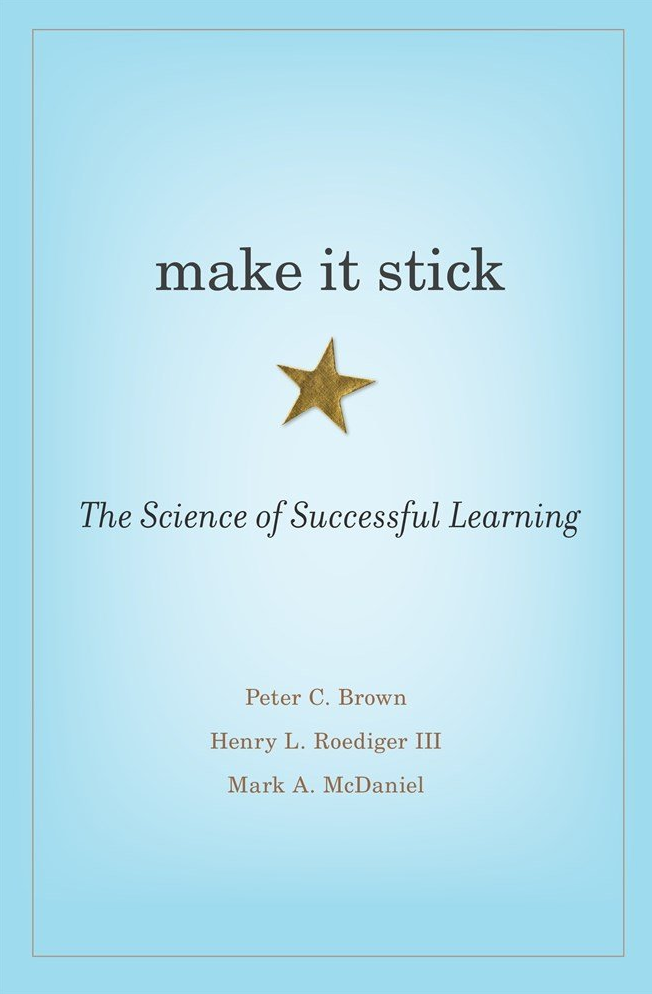
\includegraphics[width=0.15\paperwidth]{01_resources/makeitstick_frontpage.png}}
    \end{picture}
\end{frame}

\section{Outlook}
\begin{frame}{Outlook}
    \begin{enumerate}
        \item \positive{Introduction}
        \vspace{.5em}
        \item Next: \red{Illusions of Knowing}
        \item \grey{Understanding the Brain}
        \item \grey{Learning}
        \item \grey{Desirable Difficulties}
        \item \grey{Effective vs. Ineffective Learning Strategies}
        \vspace{.5em}
        \item \grey{Retrieval}
        \item \grey{Spacing}
        \item \grey{Variation and Interleaving}
        \item \grey{Mental Models}
        \item \grey{Memory Cues}
    \end{enumerate}
\end{frame}

\thankyou{Happy Learning!}{sven.ligensa@uni-muenster.de}

\sources

\end{document}
